%
%You can keep the 12pt font size, or go to 11pt or (default) 10pt
% Do NOT go any larger than 12pt font size for submission
%
%If you want to edit a printed copy, you may want to add draft mode
% (as in \documentclass[draft,conference,12pt]{IEEEtran})
% This adds space between the lines providing easier editing markup
%
%For more details see 
% http://ras.papercept.net/conferences/support/files/IEEEtran_HOWTO.pdf
%
\documentclass[conference,12pt, ]{IEEEtran}
\usepackage[margin=1truein]{geometry}
\usepackage{cite}
\usepackage{graphicx}
\usepackage{algorithmic}
\usepackage{url}
\usepackage{flushend}
\usepackage{listings}

% correct bad hyphenation here
\hyphenation{op-tical net-works semi-conduc-tor}

\begin{document}


\title{Avoiding General Purpose Microcontrollers For Multirotor Autonomous Flight }

\author{
	\IEEEauthorblockN{Innocent Niyibizi}
  \IEEEauthorblockA{Computer Science Department\\Missouri University of Science and Technology\\Rolla, MO 65409\\
  Email: iniyibizi@mst.edu}
}


% make the title area
\maketitle

\begin{abstract}
As the world continues to develop, more and more problems arise that can be solved with the use of advanced software systems. These problems can be things such as navigating an unfamiliar environment or surveying known environments after disaster strikes. To accomplish these goals, months of R\&D is poured into specific problems and how to solve them with the current technological advances. 
\end{abstract}

\section{Introduction}
This is where the introduction will go for the paper. 
	\begin{enumerate}
		\item Brief overview of the problem at hand
		\item Introduce the competition of IARC
	\end{enumerate}
This opens up the doors to many applications that can be had. A design team on campus, The Multirotor Robot Design Team is one such team and has been tackling this since 2016. They have gone through many microcontrollers and have found the feasibility of each one for the given task.

\section{History}
This is where the history of each micro controller will be brought up and the team's usage for each one. 
\begin{enumerate}
	\item APM Flight Board, not even close
	\item Arduino with no other sensors, disaster
	\item PixHawk with some sensors, getting better 
		\begin{enumerate}
			\item Sonar Sensors
		\end{enumerate}
	\item Pixhawk with sensors but trying to write low level code, Questionable
		\begin{enumerate}
			\item Optical Flow
			\item Rangefinder
			\item Lidar
		\end{enumerate}
	\item Pixhawk with sensors and built in functions, beautiful
		\begin{enumerate}
			\item Optical Flow
			\item Rangefinder
		\end{enumerate}
\end{enumerate}

\section{The Microcontrollers That Could}
\subsection{APM Flight Board: Captain}
\begin{figure}
	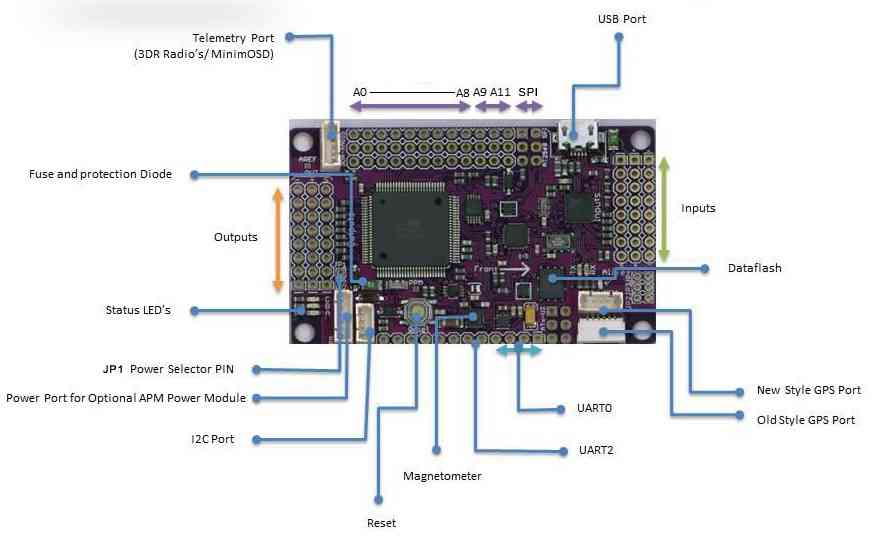
\includegraphics[scale=0.40]{apm2.jpg}
	\caption {Layout of APM2.5 Flight Controller}
\end{figure}
	\begin{enumerate}
		\item Features
		\item Use Cases
		\item Practicality of task at hand 
	\end{enumerate}

\subsection{Arduino: Mega}
\begin{figure}
	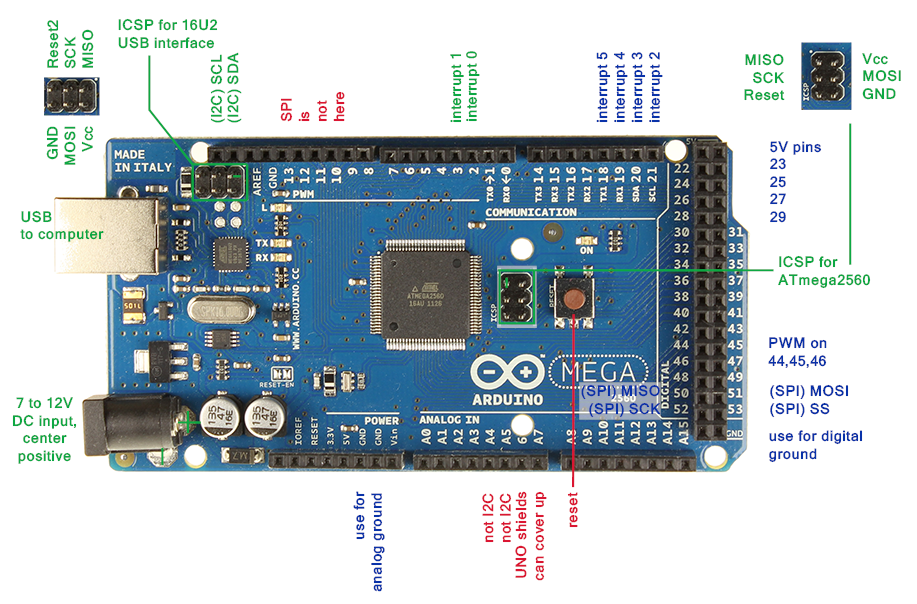
\includegraphics[scale=0.25]{mega.png}
	\caption {Layout of Arduino Mega  Microcontroller}
\end{figure}
	\begin{enumerate}
		\item Features
		\item Use Cases
		\item Practicality of task at hand 
	\end{enumerate}

\subsection{Cortex-M4: PixHawk 2 (The Cube)}
This section should include an image of the design
	\begin{enumerate}
		\item Features
		\item Use Cases
		\item Practicality of task at hand 
	\end{enumerate}


\section{Conclusion}
This section is where the paper will end and everything will make sense once again

  \begin{thebibliography}{999}

  \bibitem{linux_source} Bootlin {\em Linux source code: (v4.18.15) - Bootlin. [Online]. Available: \url{https://elixir.bootlin.com/linux/v2.6.36/source/kernel/sched.c}} [Accessed: 07-Dec-2018].

  \bibitem{virtual_runtime}  CFS Scheduler {\em [Online]. Available: \url{https://www.kernel.org/doc/Documentation/scheduler/sched-design-CFS.txt}} [Accessed: 07-Dec-2018].

  \bibitem{testing_sched} L. Jelenković, S. Groš, and D. Jakobović {\em Testing task schedulers on Linux system.} 

  \bibitem{red_black_tree} J. Morris {\em “Red Black Trees,” Data Structures and Algorithms: Hash Tables. [Online]. Available: \url{https://www.cs.auckland.ac.nz/software/AlgAnim/red_black.html}.} [Accessed: 07-Dec-2018]

  \end{thebibliography}
\end{document}

